\section{Auswertung}

\subsection{Messung der Zeitkonstanten mit einer Entladekurve}

In dem ersten Teil des Versuches wird mit dem Oszilloskop die Entladekurve des
sich im RC-Kreis befindenden Kondensators betrachtet. Dem in Abbildung \ref{fig:thermodruck}
zu sehenden Thermodruck werden dabei 13 Wertepaare, bestehend aus der Zeit $t$
und der Kondensatorspannung $U\ua{C}$, entnommen und in den Graphen
(Abbildung \ref{fig:Messunga}) eingetragen. Mithilfe einer linearen Regression nach
Formel \eqref{eqn:FitMessungA} kann dann die Steigung ermittelt werden, deren
Kehrwert im Betrag der Zeitkonstante $RC$ entspricht.

\begin{align}
  \label{eqn:FitMessungA}
  ln \left( U\ua{C} \right) &= m \cdot t + b \\
  m    &= -\frac{1}{RC}
\end{align}

\begin{table}
  \centering
  \caption{Entnommene Wertepaare für die Spannungsamplituden zu verschiedenen
          Zeitpunkten des Entladevorgangs}
  \label{tab:MessungA}
  \begin{tabular}{c c || c c}
    \toprule $t \,\, in \,\, \su{ms}$ & $U\ua{C} \,\, in \,\, \su{V}$ &
             $t \,\, in \,\, \su{ms}$ & $U\ua{C} \,\, in \,\, \su{V}$ \\
    \midrule
    0.00 & 12.4 & 1.75 & 3.4 \\
    0.25 & 10   & 2.00 & 2.8 \\
    0.50 &  8.2 & 2.25 & 2.4 \\
    0.75 &  6.6 & 2.50 & 2   \\
    1.00 &  5.8 & 2.75 & 1.8 \\
    1.25 &  4.6 & 3.00 & 1.6 \\
    1.50 &  4   & -    & -   \\
    \bottomrule
  \end{tabular}
\end{table}

Mithilfe der linearen Regression ergibt sich dabei für die Zeitkonstante $RC$ ein
Wert von:

\begin{equation}
  RC = (0.00146 \pm 0.00003) \, \su{s}.
\end{equation}

Für die Steigung m egibt sich:

\begin{equation}
  m = (-688 \pm 14) \, \frac{1}{su{s}}.
\end{equation}

\begin{figure}
  \centering
  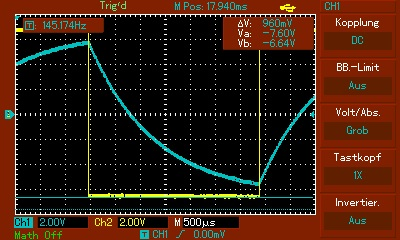
\includegraphics[width = 12 cm]{Sternchen.jpg}
  \caption{Thermodruck der in Messung 3.1 betrachteten Entladekurve }
  \label{fig:thermodruck}
\end{figure}

\begin{figure}
  \centering
  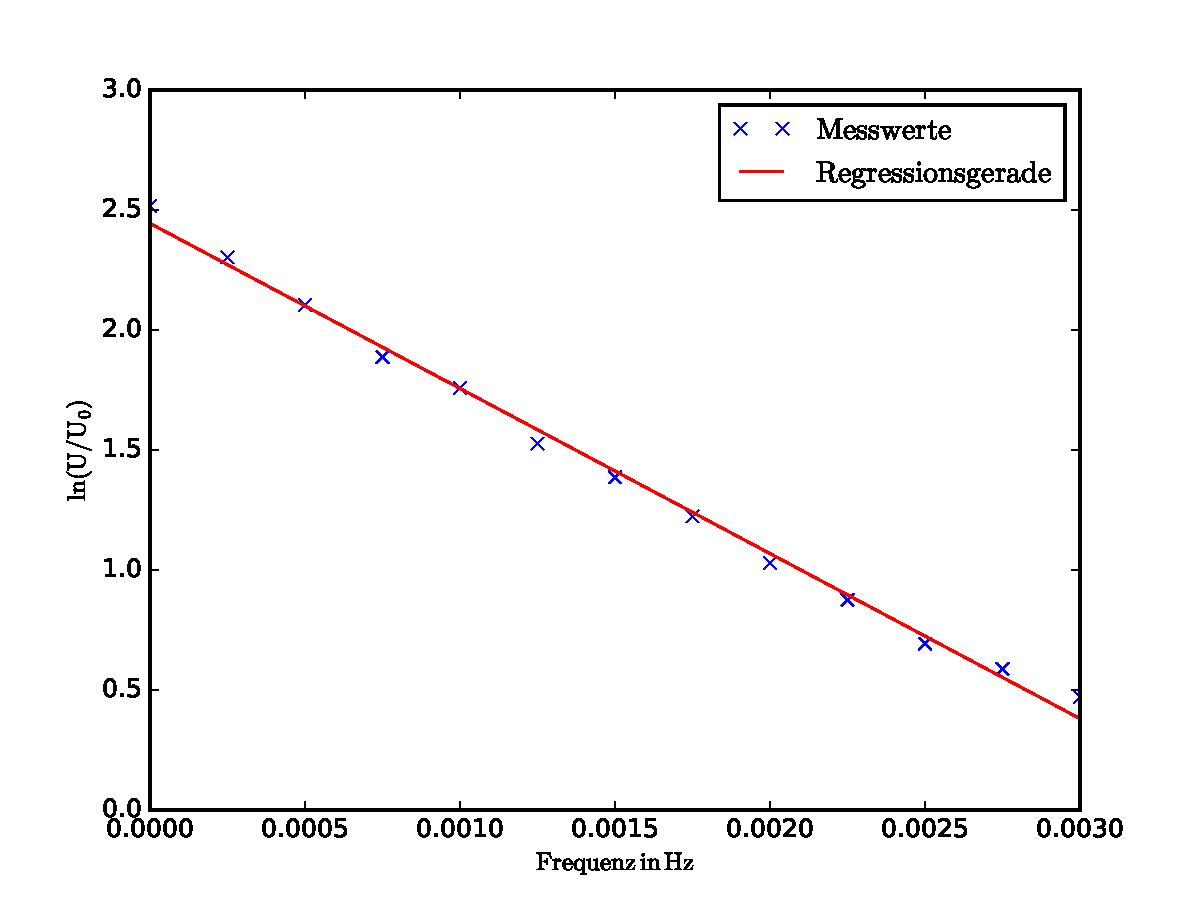
\includegraphics[width = 12 cm]{Messunga.pdf}
  \caption{Gemessene Werte für $U\ua{C}$ aufgetragen gegen die Zeit $t$}
  \label{fig:Messunga}
\end{figure}

%Eingügen der Grafik mit den eingetragenenen Werten

\newpage

\subsection{Bestimmung der Zeitkonstanten über Messung der zeitabhängigen Spannungsamplitude}

In der zweiten Messung des Versuches wurde mithilfe des Oszilloskopes die
Spannungsamplitude an dem Kondensator in Abhängigkeit der Frequenz gemessen,
da auch diese eine Abhängigkeit von der Zeitkonstante aufweist.
Das Verhältnis von gemessener Amplitude $U\ua{C}$ und der anliegenden
Ausgangsspannung wird $U\ua{G}$ in dem Graphen \ref{fig:Messungb} aufgetragen und
mithilfe einer Regressionskurve nach Formel \eqref{eqn:FitMessungB} kann dann
die Zeitkonstante RC bestimmt werden, die in Formel \eqref{eqn:FitMessungB} der
Konstante a entspricht.

\begin{equation}
  \frac{A(\nu)}{U\ua{G}} = \frac{1}{ \sqrt{ 1 + ( 2 \cdot \pi \cdot \nu )^2 \cdot a^2}}
  \label{eqn:FitMessungB}
\end{equation}

Aus der Abbildung \ref{fig:Messungb} ergibt sich somit mit der Regressionskurve
für die Zeitkonstante folgender Wert:

\begin{equation}
  RC = a = (0.00130 \pm 0.00002) \, \su{s} .
\end{equation}

\begin{figure}
  \centering
  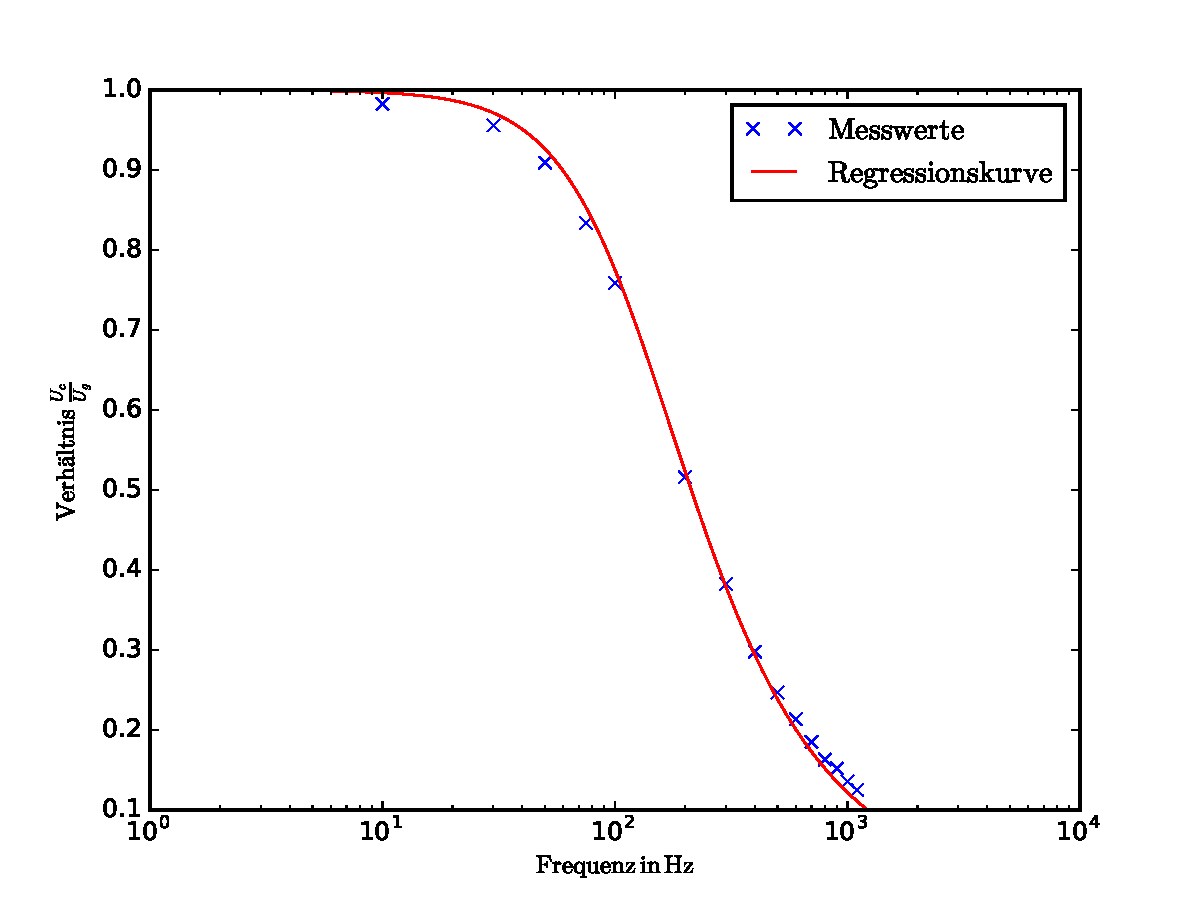
\includegraphics[width = 12 cm]{Messungb.pdf}
  \caption{Verhältnis der gemessenen Spannungsamplituden $U\ua{C}$ und der
           Ausgangsspannung $U\ua{0}$ aus Tabelle \ref{tab:MessungB} aufgetragen
          gegen die Frequenz $\nu$}
  \label{fig:Messungb}
\end{figure}

\begin{table}
  \centering
  \caption{Gemessene Spannungsamplituden der Kondensatorspannung für verschiedene
           angelegte Frequenzen $\nu$}
  \label{tab:MessungB}
  \begin{tabular}{ c c c || c c c }
    \toprule $\nu \,\, in \,\, \su{Hz}$ & $U\ua{C} \,\, in \,\, \su{V}$ & $U\ua{C} \,\, in \,\, \su{V}$ &
             $\nu \,\, in \,\, \su{Hz}$ & $U\ua{C} \,\, in \,\, \su{V}$ & $U\ua{C} \,\, in \,\, \su{V}$ \\
    \midrule
     10 & 14.1  & 14.35 &  500 & 3.48 & 14.1 \\
     30 & 13.62 & 14.25 &  600 & 3.01 & 14.1 \\
     50 & 12.91 & 14.20 &  700 & 2.61 & 14.1 \\
     75 & 11.88 & 14.25 &  800 & 2.30 & 14.1 \\
    100 & 10.77 & 14.2  &  900 & 2.14 & 14.1 \\
    200 &  7.29 & 14.13 & 1000 & 1.90 & 14.0 \\
    300 &  5.39 & 14.1  & 1100 & 1.74 & 13.9 \\
    400 &  4.20 & 14.1  & -    & -    & -    \\
    \bottomrule
  \end{tabular}
\end{table}

\subsection{Messung der Zeitkonstante über die Phasenverschiebung}

In dem dritten Teil des Experimentes wird die Zeitkonstante noch einmal über
den Phasenverschub bestimmt, der sowohl
von der Frequenz als auch von der Zeitkonstante abhängig ist. Die gemessenen Werte
für die zeitliche Verzögerung $a$ sowie die Schwingungsdauer $b$ und die daraus
resultierende Phasenverschiebung $\varphi$ sind in der folgenden Tabelle zu sehen
und wurden mithilfe eines Oszilloskopes gemessen.

\begin{table}
  \centering
  \caption{Gemessene Werte für die Parameter a und b sowie die \\ resultierende Phasenverschiebung}
  \label{tab:Phasenverschiebung}
  \begin{tabular}{c c c c}
    \toprule $\nu \,\, in  \,\, \su{Hz}$ & $a \,\, in \,\, \su{ms}$ &
             $b \,\, in \,\, \su{ms}$ & $\varphi \,\, in \,\, \su{rad}$ \\
    \midrule
     10 & 99.2 & 100.1 & 0.055 \\
     30 & 32.0 &  33.3 & 0.253 \\
     50 & 18.4 &  20.0 & 0.506 \\
     75 & 12.0 &  13.3 & 0.631 \\
    100 & 8.80 &  10.0 & 0.754 \\
    200 & 4.20 &  5.00 & 1.005 \\
    300 & 2.68 &  3.33 & 1.226 \\
    400 & 2.00 &  2.50 & 1.257 \\
    500 & 1.60 &  2.00 & 1.257 \\
    600 & 1.32 &  1.67 & 1.317 \\
    700 & 1.12 &  1.43 & 1.362 \\
    800 & 1.00 &  1.25 & 1.257 \\
    900 & 0.88 &  1.11 & 1.302 \\
    1000 & 0.76 &  1.00 & 1.508 \\
    1100 & 0.66 &  0.91 & 1.726 \\
    \bottomrule
  \end{tabular}
\end{table}

\newpage

Die gemessene Phasenverschiebung wird in Abbildung \ref{fig:Messungc} gegen die
eingestellte Frequenz aufgetragen. Über eine Regressionskurve nach Formel
\eqref{eqn:regressionC}, in der der Parameter a der zu bestimmenden Zeitkonstante
RC entspricht.

\begin{equation}
  \varphi = \arctan (- 2 \pi \nu a)
  \label{eqn:regressionC}
\end{equation}

Für RC ergibt sich somit der folgende Wert:

\begin{equation}
  RC = (0.00139 \pm 0.00013) \, \su{s} .
\end{equation}

\begin{figure}
  \centering
  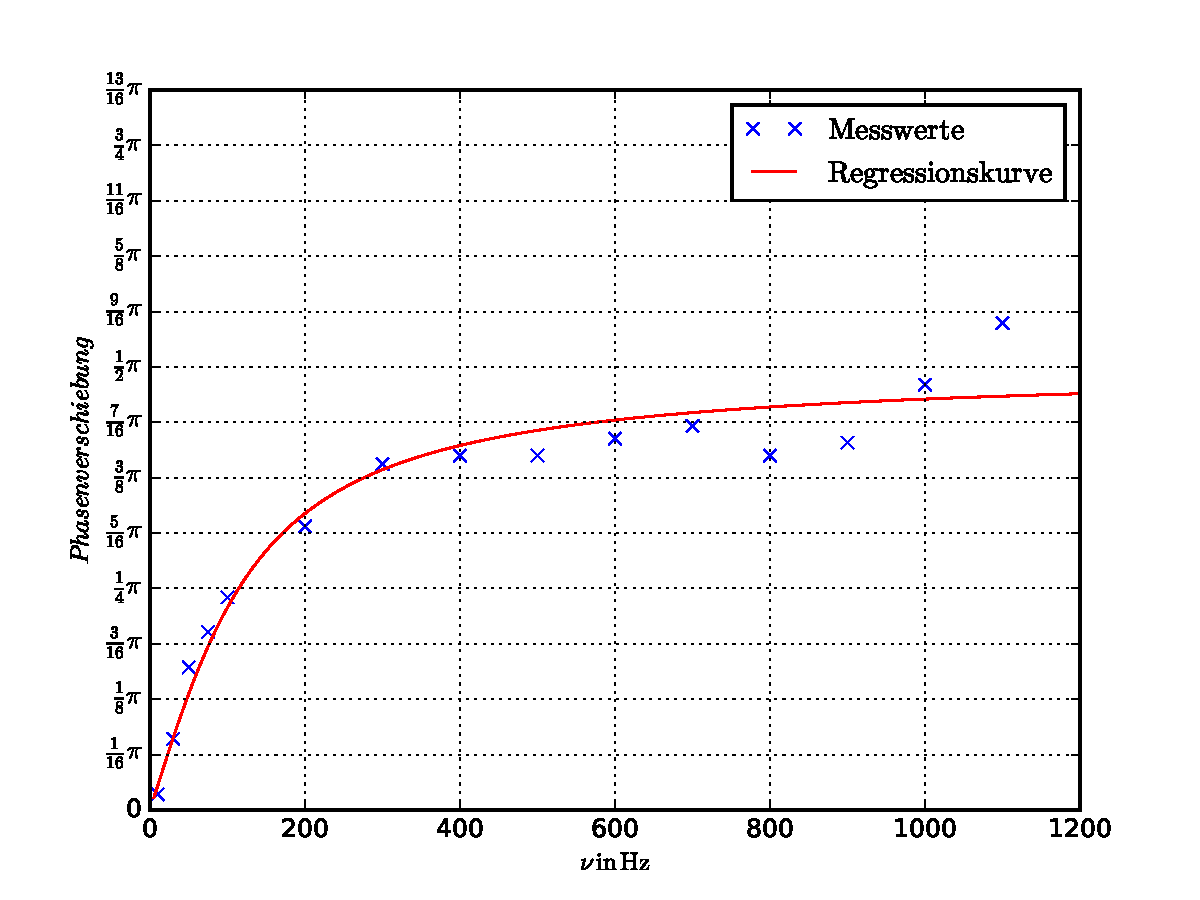
\includegraphics[width = \textwidth]{Messungc.pdf}
  \caption{Abhängigkeit der Phasenverschiebung von der angelegten Frequenz}
  \label{fig:Messungc}
\end{figure}

In Abbildung \ref{fig:Messungc} zeigt sich, dass ein Wert der Phasenverschiebung
über dem Wert $\frac{\pi}{2}$ liegt, was laut der Theorie nicht möglich sein sollte.
Deswegen wurde die Zeitkonstante noch einmal bestimmt, wobei der letzte Messwert
bei der Regression nicht beachtet wurde. Als korrigierter Wert ergibt sich somit:

\begin{equation}
  RC = (0.00136 \pm 0.00010) \, \su{s} .
\end{equation}

\subsection{Phasenabhängigkeit der Generatorspannung}

Um in diesem Abschnitt die Amplitude noch einmal als Funktion der Phasenverschiebung
zu berechnen, wird als RC der vorher berechnete Wert von $RC = (0.00136 \pm 0.00010)
\,\su{s}$ verwendet. Die berechneten Wert befinden sind in der folgenden Tabelle
sichtbar und sind in Abbildung \ref{fig:Messungd} nochmal in einem Polarplot dargestellt.

\begin{table}
  \centering
  \caption{Berechnete Amplituden aus den Werten von Aufgabenteil 3.3}
  \label{tab:AmplitudeNeu}
  \begin{tabular}{c c c }
    \toprule $\nu \,\, in  \,\, \su{Hz}$ & $\varphi \,\, in \,\, \su{rad}$
           & $\frac{A}{U\ua{G}}$ \\
    \midrule
     10 & 0.055 & 0.646 \\
     30 & 0.253 & 0.975 \\
     50 & 0.506 & 1.133 \\
     75 & 0.631 & 0.921 \\
    100 & 0.754 & 0.801 \\
    200 & 1.005 & 0.494 \\
    300 & 1.226 & 0.367 \\
    400 & 1.257 & 0.278 \\
    500 & 1.257 & 0.223 \\
    600 & 1.317 & 0.189 \\
    700 & 1.362 & 0.164 \\
    800 & 1.257 & 0.139 \\
    900 & 1.302 & 0.125 \\
    1000 & 1.508 & 0.117 \\
    1100 & 1.726 & 0.105 \\
    \bottomrule
  \end{tabular}
\end{table}

Dabei sind in Abbildung \ref{fig:Messungd} die in Tabelle \ref{tab:AmplitudeNeu}
stehenden Werte für die mit der Phasenverschiebung und der Frequenz berechneten
Amplituden eingetragen sowie zudem auch die gemessenen Amplituden in Abhängigkeit
der Frequenz aus Messung 3.2. Bei der roten Linie handelt es sich dabei um eine
zum Vergleich der Werte herangezogene Theoriekurve.

\newpage

\begin{figure}
  \centering
  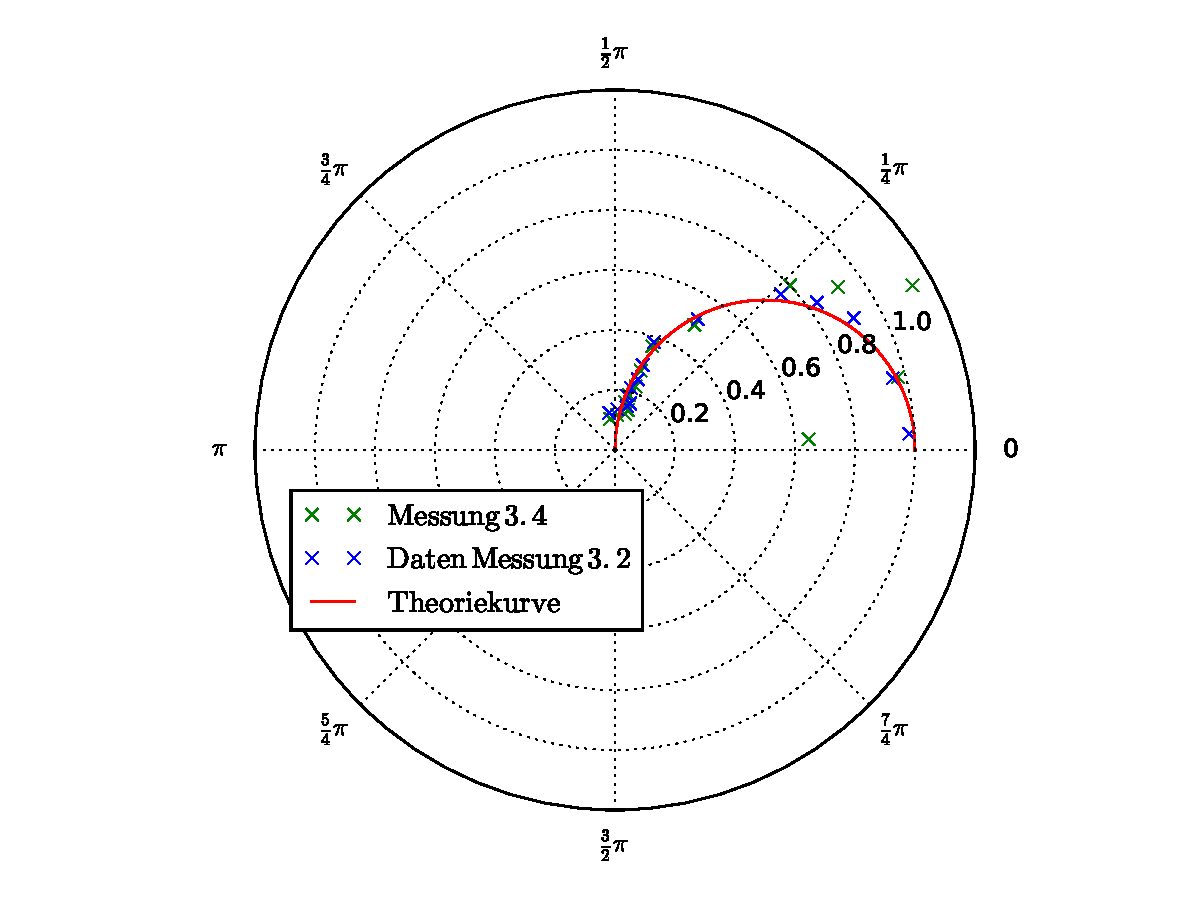
\includegraphics[width =  \textwidth]{Messungd.pdf}
  \caption{Amplitude in Abhängigkeit der Phase}
  \label{fig:Messungd}
\end{figure}


\subsection{Betrachten des RC-Kreises als Integrator}

In dem letzten Teil des Experimentes sollte mithilfe eines Oszilloskopes und drei
verschiedenen Spannungen noch einmal betrachtet werden, inwieweit der RC-Kreis
die Eigenschaften eines Integrators besitzt. In den Abbildungen \ref{fig:Rechteck}
,\ref{fig:Dreieck}  und \ref{fig:Sinus}  ist
dabei die eingespeiste Generatorspannung (gelb) sowie die Kondensatorspannun (blau)
zu erkennen.

Da bei dem ersten Thermodruck am Kreis eine Rechteckspannung anliegt, sollte bei
in Abbildung \ref{fig:Rechteck} an dem Kondensator eine Dreiecksspannung, bzw.
auf jedem Intervall eine Gerade zu erkennen sein:

\begin{equation*}
   \int c \, \su{dx}= cx+b \,\,\,\, c,b\in\su{R}.
\end{equation*}

\FloatBarrier
\begin{figure}
  \centering
  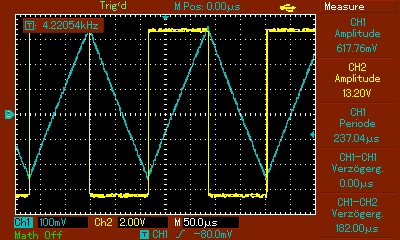
\includegraphics{Rechteck.jpg}
  \caption{Anliegende Rechteckspannung bei dem RC-Kreis}
  \label{fig:Rechteck}
\end{figure}
\FloatBarrier

Entsprechend der Integration einer Geraden sollte bei einspeisen einer Dreiecksspannung
in den RC-Kreis an dem Kondensator ein Spannungsverlauf mit periodisch aneinander
gereihten quadratischen Funktionen zu erkennen sein, was sich mit Abbildung \ref{fig:Dreieck}
auch bestätigen lässt:

\begin{equation*}
   \int mx+b \, \su{d}{x}= \frac{1}{2}mx^2+bx+c \,\,\,\, m,b,c\in\su{R}.
\end{equation*}

\begin{figure}
  \centering
  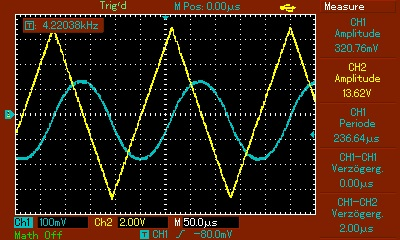
\includegraphics{Dreieck.jpg}
  \caption{Anliegende Dreieckspannung bei dem RC-Kreis}
  \label{fig:Dreieck}
\end{figure}

\newpage

Bei einer anliegenden Sinusspannung sollte sich durch den RC-Kreis entsprechend
der Integrationsregeln eine Cosinusspannung einstellen, was in Abbildung \ref{fig:Sinus}
auch beobachtbar ist:

\begin{equation*}
  \int \sin(x)\, \su{dx} = - \cos(x)+c \,\,\,\, c\in \su{R}.
\end{equation*}

\begin{figure}
  \centering
  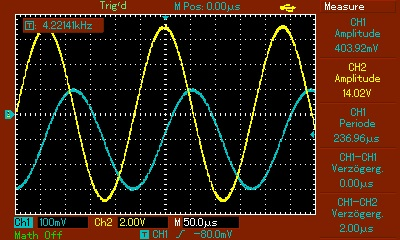
\includegraphics{Sinus.jpg}
  \caption{Anliegende Sinusspannung bei dem RC-Kreis}
  \label{fig:Sinus}
\end{figure}

\section{Diskussion}

In diesem Versuch wurden zusammengefasst drei verschiedene Methoden betrachtet,
die alle eine Bestimmung der Zeikonstante RC ermöglichten. Die verschiedenen
Messergebnisse sind in der folgenden Tabelle noch einmal aufgelistet.

\begin{table}
  \caption{Bestimmte Werte für RC bei den verschiedenen Messungen}
  \label{tab:Zusammenfassung}
  \begin{tabular}{c | c c c c}
    \toprule  $Messung$ & $3.1$ & $3.2$ & $3.3$ & $3.3 \,\, mit \,\, Korrektur$ \\
    \midrule  $RC \, \pm \, \increment RC$ & $0.00146 \, \pm \, 0.00003$ &
              $0.00130 \, \pm \, 0.00002$ & $0.00139 \, \pm \, 0.00013$ &
              $0.00136 \, \pm \, 0.00010$ \\
    \bottomrule
  \end{tabular}
\end{table}

Wie man sieht, weichen die bestimmten Werte teilweise doch deutlich von einander
ab, wobei auch die Fehlergrenzen so gering sind, dass kein Wert im Fehlerintervall
eines anderen liegt.

Ein Grund für diese Abweichungen sind vermutlich die Messmethoden. Bei der Messung
3.1 wurden zum Beispiel die verwendeten Werte einfach aus dem Thermodruck abgelesen.
Da dieser jedoch eine ziemlich geringe Auflösung besitzt, entstehen hier wahrscheinlich
schon ziemlich hohe Abweichungen zu den eigentlich gemessenen Werten.

Bei der Messung 3.2 wurde über eine Messung der Ausgangsspannung sowie der
frequenzabhängigen Amplitude die Zeitkonstante bestimmt. Vergleicht man diesen
Wert mit dem im Abschnitt 3.1 bestimmten, so ist eine starke Abweichung erkenntlich.
Betrachtet man die beiden Schaltpläne der Messungen, sieht man, dass vor allem
der hohe Innenwiderstand des Generators bei den Messungen zu Abweichungen führen
kann. Da die Amplituden mithilfe des Oszilloskopes gemessen wurden, ist eine
Ungenauigkeit durch das Ablesen eher unwahrscheinlich, jedoch spielt die Genauigkeit
des Oszilloskopes dafür eine Rolle bei den Entstehungen der Abweichungen.

%Vielleicht noch etwas einfügen zu systematischen Fehler

Wie in Abschnit 3.3 schon erwähnt, ist bei der Messung über
die Phasenverschiebung ein systematischer Fehler zu vermuten, da als Ergebnisse
Werte entstehen, die laut der Theorie nicht zulässig sind. Deswegen wurde
nochmal ein Korrekturwert ermittelt, bei dem die nach Theorie nicht zulässigen
Werte nicht beachtet wurden. Zudem ist die Entstehung der Abweichungen aufgrund
eines Ablesefehlers ziemlich wahrscheinlich, da das genaue Bestimmen des
Abstandes a besonders für kleine Werte ziemlich fehleranfällig ist.

In dem Polarplot in Abbildung \ref{fig:Messungd} sind nochmal die bestimmten Amplituden
mit den Werten aus den Messungen 3.2 und 3.3 eingetragen. Sichtbar ist, dass die
Werte aus der Messung 3.2 deutlich näher an der Theoriekurve liegen als die bestimmten
Amplituden mit den Werten aus Messung 3.3. Jedoch gilt das nur für die Werte
oberhalb eines Phasenverschubes von $\frac{\pi}{4}$.

In Abschnitt 3.5 wurde der RC-Kreis noch einmal als Integrator betrachtet. Bei allen
drei Spannungstypen zeigt sich, dass diese Beziehung bestätigt werden kann, da alle
gemessenen Darstellungen sehr mit den theoretisch ermittelten Formen für die
Spannungen übereinstimmen.
